\medskip

\textbf{Partie A : exploitation du graphique.}

\medskip

\begin{enumerate}
	\item On lit que B a pour coordonnées $(-1~;~-2)$, or la courbe $\mathcal{C}_f$ passe par B, donc $f(-1) = f(x_\mathrm{B}) = y_\mathrm{B} = -2$.

	On nous dit que la tangente $T$, tangente à $\mathcal{C}_f$ en B, d'abscisse $-1$, est aussi la droite (AB), dont le coefficient directeur est 1, donc $f'(-1) = 1$.

	\item La fonction $f$ n'est manifestement pas convexe sur son ensemble de définition, car la courbe $\mathcal{C}_f$ passe en dessous de sa tangente $T$ pour les valeurs $x$ inférieures à $- 1,7$, environ. Si la fonction était convexe sur tout son ensemble de définition, elle serait au-dessus de n'importe quelle tangente, sur tout son ensemble de définition.

Ici, on a l'impression que la fonction est d'abord concave, puis convexe, avec un point d'inflexion dont l'abscisse est aux alentours de $-1,4$.

	\item De ce que l'on peut voir de $\mathcal{C}_f$, on ne voit qu'une seule solution à l'équation, qui est environ 0,1 (à $10^{-1}$ près).
\end{enumerate}

\medskip

\textbf{Partie B : étude de la fonction $f$.}

\medskip

\begin{enumerate}
\item On a :\quad $\lim\limits_{x \to -2} x^2 + 2x - 1 = (-2)^2 + 2\times (-2) - 1 = -1$, \quad car $x\longmapsto x^2 + 2x - 1$ est une fonction polynôme, continue sur $\R$ et donc notamment continue en $-2$.

de plus :\quad $\lim\limits_{x \to -2} (x + 2) = 0$

et donc, par composition :\quad $\lim\limits_{x \to -2}\ln(x+2) = \lim\limits_{y \to 0} \ln(y) = -\infty$

finalement, par limite de la somme :\quad $\lim\limits_{x \to -2}f(x) = -\infty$.

Graphiquement, cela signifie que la courbe $\mathcal{C}_f$ admet une asymptote verticale, d'équation $x = -2$.

\item \emph{Remarque :} la justification de la dérivabilité de $f$, donnée ci-après, n'est généralement pas attendue.

\smallskip

La fonction $x \longmapsto \ln(x+2)$ est dérivable sur $]-2~;~+\infty[$, en tant que composée de $x \longmapsto x+2$ définie et dérivable sur $]-2~;~+\infty[$ et à valeurs dans $\R^{*+}$, où la fonction ln est définie et dérivable.

$f$ est dérivable sur $]-2~;~+\infty[$, en tant que somme de deux fonctions dérivables sur cet intervalle (une fonction polynôme et une fonction composée).

$\begin{aligned} \forall x \in ]-2~;~+\infty[,\quad f'(x)&=2x + 2 + 0 + \dfrac{1}{x+2}\\
&=\dfrac{(2x + 2)(x+2) + 1}{x+2}\\
&=\dfrac{2x^2 + 4x + 2x + 4 + 1}{x+2}\\
&=\dfrac{2 x^{2} + 6x + 5}{x + 2}.\end{aligned}$

On arrive bien à l'expression attendue pour la fonction dérivée $f'$.
\item Pour tout $x$ réel strictement supérieur à $-2$, $x + 2$ est strictement positif, donc le signe de $f'(x)$ est le signe de son numérateur. Ledit numérateur étant une expression polynomiale de degré 2 ayant un coefficient dominant (2) positif, cela signifie que les images seront positives, sauf entre d'éventuelles racines.

Déterminons le discriminant du numérateur: \quad $\Delta = 6^2 - 4\times 2 \times 5 = 36 - 40 = -4 <0$.

Le trinôme n'a donc pas de racines réelles, et a donc des images strictement positives pour tout $x$ réel.

$f'$ est donc une fonction à valeurs strictement positives sur $]-2~;~+\infty[$, et $f$ est donc strictement croissante sur $]-2~;~+\infty[$.

On peut donc établir le tableau de variations suivant :

	\hfill~\begin{tikzpicture}
		\tkzTabInit[lgt=3,espcl=3.5]{$x$/0.7, signe de $f'(x)$/0.7, variations de $f$/1.5}{$-2$,$+\infty$}
		\tkzTabLine{d,+,}
		\tkzTabVar{D-/$-\infty$,+/$+\infty$}
	\end{tikzpicture}\hfill~

\item La fonction $f$ est continue (car dérivable) sur $]-2~;~+\infty[$, de plus, elle est strictement croissante sur cet intervalle et enfin, 0 est une valeur intermédiaire entre $\lim\limits_{-2}f = -\infty$ ~~et~~ $\lim\limits_{+\infty}f = + \infty$.

D'après le corollaire du théorème des valeurs intermédiaires appliqué aux fonctions strictement monotones, l'équation $f(x) = 0$ admet une unique solution sur $]- 2~;~+\infty[$, que l'on notera $\alpha$.

Avec une exploration à la calculatrice (éclairée par notre lecture graphique de la partie A), on trouve $0,115 < \alpha < 0,12$, donc une valeur approchée à $10^{-2}$ de $\alpha$ est $1,12$.

\item Puisque $f$ est strictement croissante sur $]-2~;~+\infty[$, on a :

$\begin{aligned} -2 < x <\alpha &\implies f(x) < f(\alpha)\\
&\implies f(x) < 0\end{aligned}$ \hfill
$\begin{aligned} \alpha <x  &\implies  f(\alpha) < f(x)\\
&\implies 0< f(x) \end{aligned}$\hfill~

$f$ est donc à valeurs strictement négatives sur $]-2~;~\alpha[$, nulle pour $x = \alpha$ et à valeurs strictement positives sur $]\alpha~;~+\infty[$.

\item Pour étudier la présence d'un point d'inflexion, on va étudier le signe de la dérivée seconde de $f$, notée $f''$.

$f$ est deux fois dérivable sur $]-2~;~+\infty[$, car sa dérivée première est une fraction rationnelle, et donc $f'$ est dérivable partout où elle est définie.

$\begin{aligned} \forall x \in ]-2~;~+\infty[,\quad f''(x) &= \dfrac{(4x + 6)\times (x+2) - (2x^2 + 6x + 5)\times 1}{(x+2)^2}\\
&=\dfrac{4x^2+8x+6x+12-2x^2-6x-5}{(x+2)^2}\\
&=\dfrac{2x^2 +8x +7}{(x+2)^2}
\end{aligned}$

Pour tout $x$ réel strictement supérieur à $-2$, $(x+2)^2$ est une quantité strictement positive, donc le signe de $f''(x)$ est le signe de son numérateur, un polynôme de degré 2, dont le coefficient dominant est strictement positif, dont les images sont strictement positives, sauf entre ses deux éventuelles racines.

Le discriminant est :\quad $\Delta = 8^2 - 4\times 2 \times 7 = 8\times 8- 8\times 7 = 8>0$.

Le trinôme a exactement deux racines réelles distinctes, et donc s'annule en changeant de signe deux fois, pour :

$x_1 = \dfrac{-8 - \sqrt{8}}{2\times 2} = \dfrac{-8 - 2\sqrt{2}}{4} = -2 - \dfrac{\sqrt{2}}{2}$.

$x_2 = \dfrac{-8 + \sqrt{8}}{2\times 2} = \dfrac{-8 + 2\sqrt{2}}{4} = -2 + \dfrac{\sqrt{2}}{2}$.

La valeur $x_1$ est manifestement strictement inférieure à $-2$, et donc :

Sur $ \left]-2~;~-2 + \dfrac{\sqrt{2}}{2}\right[ $, $f''$ est à valeurs strictement négatives, on a $f''\left(-2 + \dfrac{\sqrt{2}}{2}\right) =0$ et sur $\left]-2 + \dfrac{\sqrt{2}}{2}~;~+\infty\right[$, $f''$ est à valeurs strictement positives.

Ainsi, $f$ est concave sur $\left]-2~;~-2 + \dfrac{\sqrt{2}}{2}\right[$ et convexe sur $\left]-2 + \dfrac{\sqrt{2}}{2}~;~+\infty\right[$ et donc son unique point d'inflexion est le point d'abscisse $-2 + \dfrac{\sqrt{2}}{2}$.

\emph{Remarque :} On a :\quad$ -2 + \dfrac{\sqrt{2}}{2}\approx-1,29$, ce qui n'est pas incohérent avec l'estimation graphique formulée en partie A dans ce corrigé.

\end{enumerate}


\textbf{Partie C : une distance minimale.}

\medskip

\begin{enumerate}
\item Le point J a pour coordonnées $(0~;~1)$ et $M$ a pour coordonnées $\big(x~;~g(x)\big)$.

Comme on est dans un repère orthonormé, on a :\quad $\mathrm{J}M = \sqrt{(x_M - x_\mathrm{J})^2 + (y_M - y_\mathrm{J})^2}$

Donc, \quad $\begin{aligned}[t] \forall x \in ]-2~;~+\infty[,\quad h(x)&=\mathrm{J}M^2\\
	&=(x_{M} - x_{\mathrm{J}})^2 + (y_{M} - y_{\mathrm{J}})^2\\
	&=(x - 0)^2 + \big(g(x) - 1\big)^2\\
	&=x^{2}+\big[\ln (x+2)-1\big]^{2}.\end{aligned}$

On arrive bien à l'expression attendue.

\item \begin{enumerate}
	\item La fonction racine carrée est strictement croissante sur $\R^+$, et la distance $\mathrm{J}M$ est nécessairement positive, en tant que distance.

Donc $\mathrm{J}M_{x_1} \leqslant \mathrm{J}M_{x_2} \iff \mathrm{J}M_{x_1}^2 \leqslant \mathrm{J}M_{x_2}^2$.

La distance $\mathrm{J}M$ sera donc minimale pour la valeur $x$ qui rend minimale le carré de cette distance, c'est-à-dire $h(x)$.
	
On sait que, pour tout $x$ dans $]-2~;~+\infty[$, $\dfrac{2}{x+2}$ est strictement positif, donc $h'(x)$ est du signe de $f(x)$.

On peut donc établir le tableau suivant :

	\hfill~\begin{tikzpicture}
			\tkzTabInit[lgt=3,espcl=3]{$x$/0.7, signe de $f(x)$/0.7,signe de $h'(x)$/0.7, variations de $h$/1.5}{$-2$,$\alpha$,$+\infty$}
			\tkzTabLine{d,-,z,+,}
			\tkzTabLine{d,-,z,+,}
			\tkzTabVar{D+/~,-/$h(\alpha)$,+/~}
	\end{tikzpicture}\hfill~

	\item Comme $h$ est décroissante sur $]-2~;~\alpha[$ et croissante sur $]\alpha~;~+\infty[$, la valeur de $x$ pour laquelle la distance $\mathrm{J}M$ est minimale est donc bien le nombre $\alpha$, solution de l'équation $f(x) = 0$, défini à la question \textbf{4.} de la \textbf{partie B}.
\end{enumerate}

\item \begin{enumerate}
	\item On sait que $\alpha$ est la solution de l'équation $f(x) = 0$.

	$\begin{aligned} f(x) = 0 &\iff x^2 + 2x - 1 + \ln(x+2) = 0\\
	&\iff \ln(x+2) = 1 - 2x -x^2 \end{aligned}$

	Comme $\alpha$ est solution de cette équation, on en déduit bien :

	$\ln (\alpha+2)=1-2 \alpha-\alpha^{2}$.

	\item La tangente à $\mathcal{C}_g$ au point $M_\alpha$ a pour coefficient directeur :\quad $g'(\alpha) = \dfrac{1}{\alpha + 2}$.

	La droite (J$M_\alpha$) a pour coefficient directeur :

	$\dfrac{y_{M_\alpha} - y_\mathrm{J}}{x_{M_\alpha} - x_\mathrm{J}} = \dfrac{g(\alpha) - 1}{\alpha - 0} = \dfrac{\ln(\alpha + 2)-1}{\alpha} = \dfrac{1 - 2\alpha - \alpha^2 - 1}{\alpha} = \dfrac{\alpha (-2 - \alpha)}{\alpha } = -2 - \alpha$.

	Le produit de ces deux coefficients directeurs est donc : \quad $\dfrac{1}{\alpha + 2}\times (-2-\alpha)~=~ -1$.

	On en déduit dont que la tangente à $\mathcal{C}_{g}$ au point $M_{\alpha}$ et la droite $\left(\mathrm{J}M_{\alpha}\right)$ sont perpendiculaires.

	\emph{Remarque :} on aurait aussi pu mobiliser des connaissances du programme de première et utiliser des vecteurs normaux ou des vecteurs directeurs de ces deux droites, et en calculer le produit scalaire (entre les deux vecteurs directeurs, ou entre les deux vecteurs normaux) ou vérifier la colinéarité (entre le vecteur directeur de l'une et le vecteur normal de l'autre), pour arriver à la même conclusion.
\end{enumerate}
\end{enumerate}
